\chapter{Extras}
The Extras menu contains features that do not deal with items created for your campaign. The Charm Cascades module provides convenient access to the entire charm database, while the preferences dialog gives you some degree of freedom on the program's basic behaviour.

\section{Charm Cascades}
The Charm Cascades module allows you to browse the entire Anathema Charm database without being limited to those charms available to your character. Currently, Charms for the supported character types as well as Sidereal Exalted are included.

\subsection{Using charm cascades}
To view the Charm Cascades, either press the yellow button in the toolbar (it vaguely resembles a Solar Charm icon) or select "Show Charm Cascades" from the ``Extras'' menu. 

\begin{figure}[htb]
	\centering
		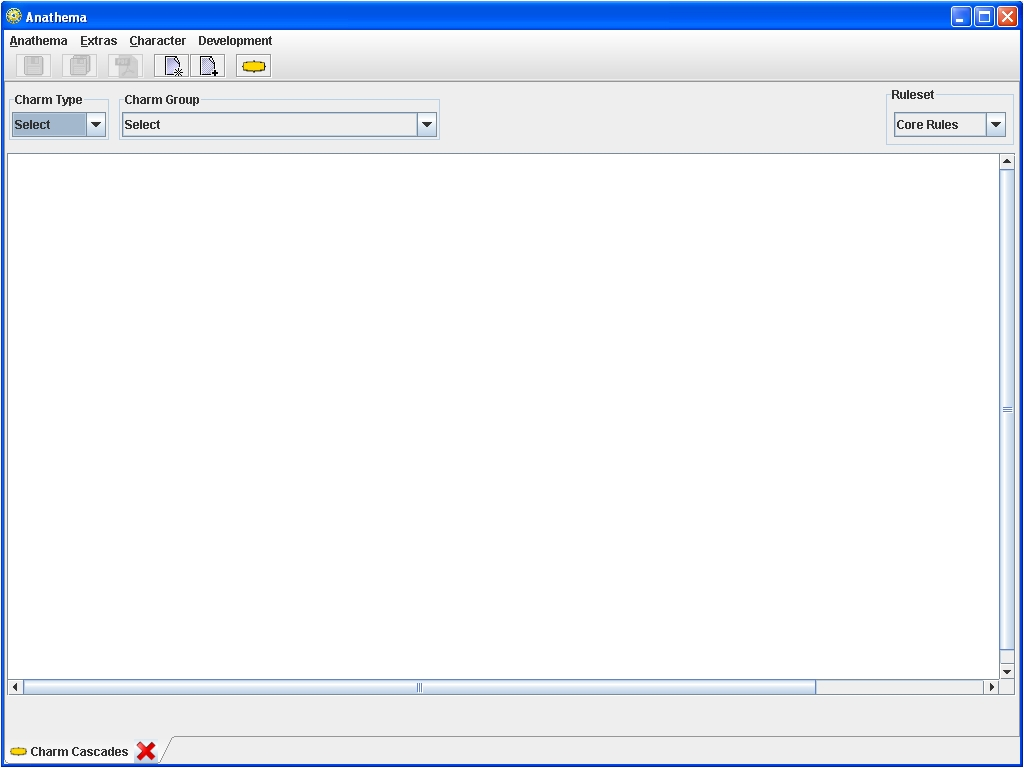
\includegraphics[width=1.00\textwidth]{Images/CharmCascadesEmpty.jpg}
	\caption{Charm Cascades view, immaculate}
	\label{fig:CharmCascadesEmpty}
\end{figure}

A new Tab will open, as depicted in figure \ref{fig:CharmCascadesEmpty}. Within, you will see three drop-down lists at the top and a vast, empty area below. Use the first drop-down, ``Charm Type``, to switch between the various character types and Martial Arts. Once done, the second drop-down box will be filled with the various charm groups for the type selected.

At a moments notice, the background of the canvas will change to the selected types color, shortly after, the charm tree for the selected group will be displayed. The graphics are closely modeled after the examples given in the Exalted rulebooks, so you should have no trouble finding your way around.

\begin{figure}[htb]
	\centering
		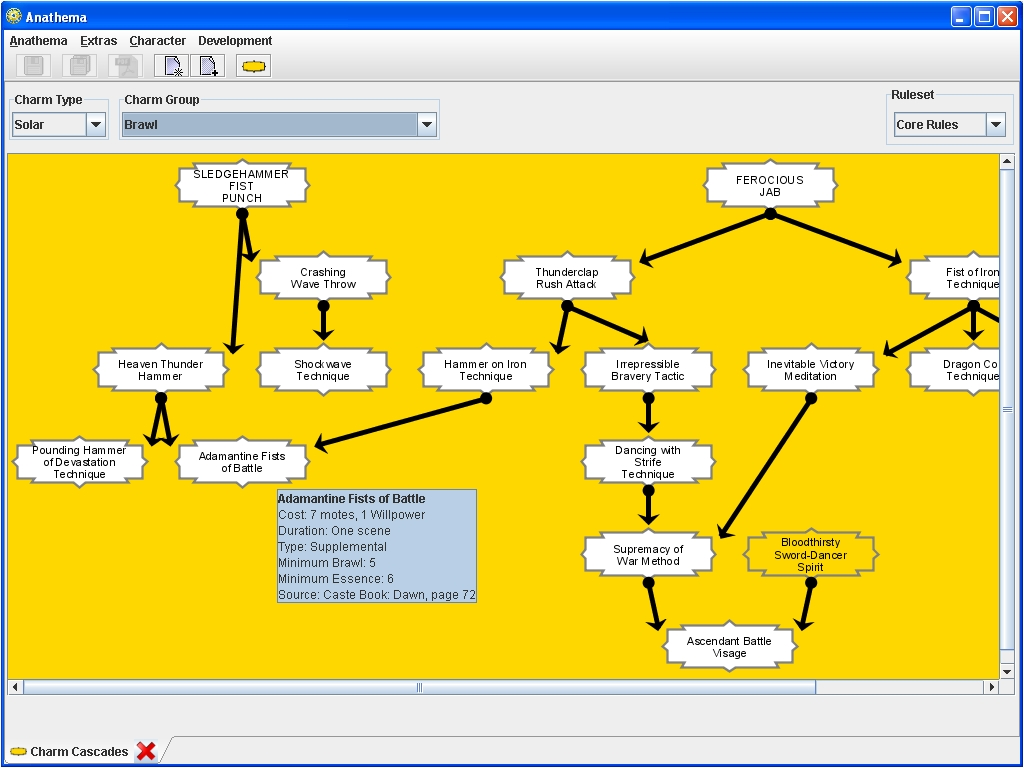
\includegraphics[width=1.00\textwidth]{Images/CharmCascadesTooltip.jpg}
	\caption{Charm Cascades view, tooltip showing}
	\label{fig:CharmCascadesTooltip}
\end{figure}

The only difference between Anathema's rendition and those familiar depictions is the way Charms from groups different than the current one are displayed: To clearly mark these 'external' charms, they are rendered not in white, but with a transparent background. An example of this can be seen at the lower right of figure \ref{fig:CharmCascadesTooltip}.

You can hover the mouse cursor over any of the charm symbols to trigger a tooltip with closer information on that charm: The entire block of statistics as well as a source are given. Refer to figure \ref{fig:CharmCascadesTooltip} for a rough impression. 'External' charms won't display any information.

The exact content displayed in the tooltip depends on the ruleset chosen, which is done by the third box above. Current selections include the Core Rules and the changes wrought by the introduction of Power Combat.

\section{Preferences}
The preferences dialog allows you to customize various aspects of Anathema. Please see section \ref{sec:Preferences} for a detailed explanation of the various options.